\documentclass[tikz,12pt]{standalone}

\usepackage{amsmath,amsfonts,amssymb,amsthm}
\usepackage{mathptmx}
\usepackage{tikz}
\usepackage{xcolor}

\definecolor{ocre}{RGB}{25,102,243} % blue
\definecolor{bole}{rgb}{0.8, 0.0, 0.0} % brown
\usetikzlibrary{patterns}
\usetikzlibrary{arrows}

\begin{document}

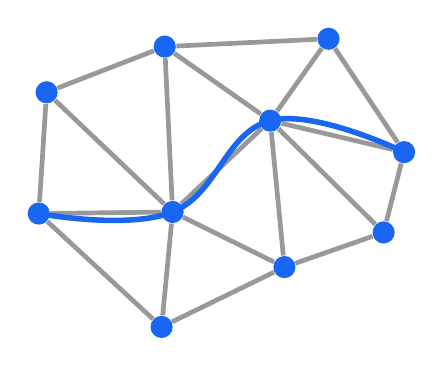
\begin{tikzpicture}
\tikzstyle{nodeBlue} = [
  shape=circle, 
  minimum size=8pt,
  inner sep=0pt,
  fill = ocre
]
\tikzstyle{tedge} = [
  draw = black!40,
  line width = 1.7
]

\node [nodeBlue] (v1) at (4.28,-4.98) {};
\node [nodeBlue] (v2) at (4.42,-3.52) {};
\node [nodeBlue] (v3) at (5.84,-4.22) {};
\node [nodeBlue] (v4) at (5.66,-2.36) {};
\node [nodeBlue] (v5) at (2.72,-3.54) {};
\node [nodeBlue] (v6) at (2.82,-2.) {};
\node [nodeBlue] (v7) at (4.32,-1.42) {};
\node [nodeBlue] (v8) at ((7.1,-3.78) {};
\node [nodeBlue] (v9) at (7.36,-2.76) {};
\node [nodeBlue] (v10) at (6.4,-1.32) {};

\draw[tedge]  (v1) -- (v2);
\draw[tedge]  (v2) -- (v3);
\draw[tedge]  (v3) -- (v1);
\draw[tedge]  (v2) -- (v4);
\draw[tedge]  (v4) -- (v3);
\draw[tedge]  (v5) -- (v1);
\draw[tedge]  (v5) -- (v6);
\draw[tedge]  (v6) -- (v2);
\draw[tedge]  (v2) -- (v5);
\draw[tedge]  (v7) -- (v6);
\draw[tedge]  (v2) -- (v7);
\draw[tedge]  (v4) -- (v8);
\draw[tedge]  (v8) -- (v3);
\draw[tedge]  (v9) -- (v8);
\draw[tedge]  (v10) -- (v7);
\draw[tedge]  (v7) -- (v4);
\draw[tedge]  (v10) -- (v9);
\draw[tedge]  (v9) -- (v4);
\draw[tedge]  (v4) -- (v10);


\draw[line width = 2, ocre] plot[smooth, tension=.7] coordinates {(v5) (v2) (v4) (v9)};

\end{tikzpicture}

\end{document}